\begin{frame}
  \frametitle{Resultados conocidos para resolver la Pregunta N$^{\circ}$1}

  \begin{theorem}[El Principio de Inducción Matemática]
    Sea $F$ un \alert{cuerpo ordenado}.
    Suponga que $\forall n\in\mathbb{N}_{F}$, $p\left(n\right)$ es
    una proposición acerca de $n$.
    Si

    \begin{multicols}{2}
      \begin{enumerate}[(1)]
        \item\label{hyp:1}

        $p\left(1\right)$ es verdadero, y

        \item\label{hyp:2}

        $\forall k\in\mathbb{N}_{F}$,
        $p\left(k\right)\implies p\left(k+1\right)$,
      \end{enumerate}
    \end{multicols}

    entonces $\forall n\in\mathbb{N}_{F}$, $p\left(n\right)$ es
    verdadero.
  \end{theorem}

  \begin{proof}
    Suponga que $p\left(n\right)$ es como se describe en la
    hipótesis.
    Sea
    \begin{math}
      A=
      \left\{
      x\in\mathbb{N}_{F}:
      p\left(x\right)\text{ es verdadero}
      \right\}
    \end{math}.
    Entonces,
    \begin{enumerate}[(i)]
      \item

            $1\in A$, por~\eqref{hyp:1}.

      \item

            Suponga que $x\in A$. Entonces, $x\in\mathbb{N}_{F}$ y
            $p\left(x\right)$ es verdadero.
            Así, por~\eqref{hyp:2}, $p\left(x+1\right)$ es verdadero.
            Esto es, $x+1\in A$.
            Por lo tanto, $x\in A\implies x+1\in A$.
            Finalmente, $A$ es conjunto inductivo y
            $\mathbb{N}_{F}\subset A$.
            Esto es, $\forall n\in\mathbb{N}_{F}$, $p\left(n\right)$
            es verdadero.
    \end{enumerate}
  \end{proof}

  \begin{definition}[Sucesión acotada]
    Una sucesión $\left\{x_{n}\right\}$ es \alert{acotada} si el
    conjunto $\left\{x_{n}:n\in\mathbb{N}\right\}$ es un conjunto
    acotado.
    Hay dos maneras equivalentes de decir que $\left\{x_{n}\right\}$
    es \alert{acotada}:
    \begin{multicols}{2}
      \begin{enumerate}[(1)]
        \item

              $\exists a,b\in\mathbb{R}$ tal que
              $\forall n\in\mathbb{N}$, $a\leq x_{n}\leq b$.

        \item

              $\exists M>0$ tal que $\forall n\in\mathbb{N}$,
              $\left|x_{n}\right|\leq M$.
      \end{enumerate}
    \end{multicols}
  \end{definition}
\end{frame}

\begin{frame}
  \begin{definition}[Sucesiones monótonas]
    Una sucesión $\left\{a_{n}\right\}$ es
    \begin{enumerate}[a)]
      \item

            \alert{monótona creciente} sii $\forall n\in\mathbb{N}$,
            $a_{n}\leq a_{n+1}$; esto es

            \begin{equation*}
              a_{1}\leq
              a_{2}\leq
              \cdots\leq
              a_{n}\leq
              a_{n+1}\leq
              \cdots.
            \end{equation*}

      \item

            \alert{monótona decreciente} sii
            $\forall n\in\mathbb{N}$, $a_{n}\geq a_{n+1}$; esto es

            \begin{equation*}
              a_{1}\geq
              a_{2}\geq
              \cdots\geq
              a_{n}\geq
              a_{n+1}\geq
              \cdots.
            \end{equation*}

      \item

            \alert{estrictamente creciente} sii
            $\forall n\in\mathbb{N}$, $a_{n}<a_{n+1}$; esto es

            \begin{equation*}
              a_{1}<
              a_{2}<
              \cdots<
              a_{n}<
              a_{n+1}<
              \cdots.
            \end{equation*}

      \item

            \alert{estrictamente decreciente} sii $\forall n\in\mathbb{N}$,
            $a_{n}>a_{n+1}$; esto es

            \begin{equation*}
              a_{1}>
              a_{2}>
              \cdots>
              a_{n}>
              a_{n+1}>
              \cdots.
            \end{equation*}
    \end{enumerate}
  \end{definition}

  \begin{example}[Estrictamente creciente]
    % https://www.math.drexel.edu/~prs49/ewExternalFiles/Monotone.pdf
    La sucesión $\left\{f\left(n\right)\right\}$, donde
    $f\left(n\right)=\arctan\left(n\right)$ es
    \alert{estrictamente creciente} porque
    \begin{math}
      \forall n\in\mathbb{N},
      f^{\prime}\left(n\right)=
      \dfrac{1}{1+n^2}>0
    \end{math}.
  \end{example}
\end{frame}

\begin{frame}
  \begin{theorem}[Convergencia Monótona para sucesiones]
    Cualquier sucesión monótona y acotada \alert{converge}.
    Más precisamente,

    \begin{enumerate}[a)]
      \item

            Si $\left\{a_{n}\right\}$ es una sucesión monótona
            creciente que es acotada superiormente, entonces el
            \begin{math}
              \lim\limits_{n\to\infty}a_{n}=
              \sup\left\{a_{n}:n\in\mathbb{N}\right\}
            \end{math}.

      \item

            Si $\left\{a_{n}\right\}$ es una sucesión monótona
            decreciente que es acotada inferiormente, entonces el
            \begin{math}
              \lim\limits_{n\to\infty}a_{n}=
              \inf\left\{a_{n}:n\in\mathbb{N}\right\}
            \end{math}.
    \end{enumerate}
  \end{theorem}

  \begin{proof}
    \begin{enumerate}[a)]
      \item

            Suponga que $\left\{a_{n}\right\}$ es acotada y monótona
            creciente.
            Dado que $\left\{a_{n}\right\}$ es acotada, el conjunto
            $\left\{a_{n}:n\in\mathbb{N}\right\}$ tiene una cota
            superior.
            Por la completitud de $\mathbb{R}$,
            \begin{math}
              \exists u=
              \sup\left\{a_{n}:n\in\mathbb{N}\right\}
            \end{math}.

            Sea $\varepsilon>0$.
            Por el criterio $\varepsilon$ para el supremo,
            $\exists n_{0}\in\mathbb{N}$ tal que $a_{n_{0}}>u-\varepsilon$.
            Pero $\left\{a_{n}\right\}$ es monótona creciente, por lo tanto,
            $n\geq n_{0}\implies a_{n}\geq a_{n_{0}}$.
            Así,
            \begin{equation}\label{eq:increasing}
              n\geq n_{0}\implies a_{n}\geq a_{n_{0}}>u-\varepsilon.
            \end{equation}

            Pero, dado que $u=\sup\left\{a_{n}:n\in\mathbb{N}\right\}$,
            \begin{equation}\label{eq:upperbound}
              \forall n\in\mathbb{N}, a_{n}\leq u.
            \end{equation}
            Juntando~\eqref{eq:increasing} y~\eqref{eq:upperbound}, tenemos
            \vspace*{-.3cm}
            \begin{align*}
              n\geq n_{0}
               & \implies u-\varepsilon<a_{n}\leq u< u+\varepsilon \\
               & \implies u-\varepsilon<a_{n}<u+\varepsilon        \\
               & \implies \left|a_{n}-u\right|<\varepsilon.
            \end{align*}
            Por lo tanto,
            \begin{math}
              \lim\limits_{n\to\infty}a_{n}=
              u=
              \sup\left\{a_{n}:n\in\mathbb{N}\right\}
            \end{math}.
      \item De manera análoga.
    \end{enumerate}
  \end{proof}
\end{frame}

\begin{frame}
  \begin{corollary}[Teorema Fundamental de las Sucesiones Monótonas]
    Una sucesión monótona converge sii esta es es acotada.
  \end{corollary}

  \begin{theorem}[Teorema de Bolzano-Weierstraß para sucesiones]
    \label{thm:bolzano-weierstraß}
    Cualquier sucesión acotada tiene una subsucesión convergente.
  \end{theorem}

  \begin{proof}
    \begin{enumerate}
      \item

            Suponga cualquier sucesión acotada.

      \item

            Cree el intervalo cerrado inicial cuyos extremos son
            dichas cotas y construya una sucesión de intervalos
            encajados.

      \item

            Use el teorema de intervalos encajados de Cantor y
            concluya que existe un único número real en la
            intersección.

      \item

            Pruebe que la subsucesión converge a ese número real.
    \end{enumerate}
  \end{proof}

  \begin{theorem}
    Una sucesión acotada es convergente sii tiene uno y solo un punto
    de acumulación.
  \end{theorem}

  \begin{proof}
    Para el recíproco use el teorema~\ref{thm:bolzano-weierstraß} y
    por contradicción.
  \end{proof}
\end{frame}

\begin{frame}
  \begin{definition}[Funciones monótonas]
    Una función $f$ es
    \begin{enumerate}[(a)]
      \item\label{mon:increasing}

      \alert{monótona creciente} en un conjunto
      $A\subset\mathcal{D}\left(f\right)$ sii
      $\forall x_{1},x_{2}$ en $A$,

      \begin{equation*}
        x_{1}<
        x_{2}\implies
        f\left(x_{1}\right)\leq
        f\left(x_{2}\right);
      \end{equation*}

      \item\label{mon:decreasing}

      \alert{monótona decreciente} en un conjunto
      $A\subset\mathcal{D}\left(f\right)$ sii
      $\forall x_{1},x_{2}$ en $A$,

      \begin{equation*}
        x_{1}<
        x_{2}\implies
        f\left(x_{1}\right)\geq
        f\left(x_{2}\right);
      \end{equation*}

      \item\label{mon:strict-increasing}

      \alert{estrictamente creciente} en un conjunto
      $A\subset\mathcal{D}\left(f\right)$ sii
      $\forall x_{1},x_{2}$ en $A$,

      \begin{equation*}
        x_{1}<
        x_{2}\implies
        f\left(x_{1}\right)<
        f\left(x_{2}\right);
      \end{equation*}

      \item\label{mon:strict-decreasing}

      \alert{estrictamente decreciente} en un conjunto
      $A\subset\mathcal{D}\left(f\right)$ sii
      $\forall x_{1},x_{2}$ en $A$,

      \begin{equation*}
        x_{1}<
        x_{2}\implies
        f\left(x_{1}\right)>
        f\left(x_{2}\right);
      \end{equation*}

      \item

            \alert{monótona} en $A\subset\mathcal{D}\left(f\right)$
            si este satisface~\eqref{mon:increasing}
            o~\eqref{mon:decreasing}
            y \alert{estrictamente monótona} en
            $A\subset\mathcal{D}\left(f\right)$ si este satisface
            satisface~\eqref{mon:strict-increasing}
            o~\eqref{mon:strict-decreasing}.
    \end{enumerate}
  \end{definition}

  \begin{example}[Estrictamente creciente]
    % https://www.math.drexel.edu/~prs49/ewExternalFiles/Monotone.pdf
    La función $f$, donde
    $f\left(x\right)=\arctan\left(x\right)$ es
    \alert{estrictamente creciente} porque
    \begin{math}
      \forall x\in\mathbb{R},
      f^{\prime}\left(x\right)=
      \dfrac{1}{1+x^2}>0
    \end{math}.
  \end{example}
\end{frame}

\begin{frame}
  \begin{theorem}
    Suponga que $f$ es diferenciable sobre un intervalo $I$.
    \begin{enumerate}[(a)]
      \item\label{crit:increasing}

      Si $f^{\prime}\left(x\right)\geq 0$, $\forall x\in I$, entonces
      $f$ es monótona creciente sobre $I$.

      \item\label{crit:decreasing}

      Si $f^{\prime}\left(x\right)\leq 0$, $\forall x\in I$, entonces
      $f$ es monótona decreciente sobre $I$.

      \item\label{crit:strict-increasing}

      Si $f^{\prime}\left(x\right)>0$, $\forall x\in I$, entonces
      $f$ es estrictamente creciente sobre $I$.

      \item\label{crit:strict-decreasing}

      Si $f^{\prime}\left(x\right)<0$, $\forall x\in I$, entonces
      $f$ es estrictamente decreciente sobre $I$.
    \end{enumerate}
  \end{theorem}

  \begin{alertblock}{Tener cuidado}
    Las reciprocas de~\eqref{crit:strict-increasing}
    y~\eqref{crit:strict-decreasing} son falsas.
  \end{alertblock}

  \begin{proof}
    Suponga que $f$ es diferenciable sobre un intervalo $I$.
    \begin{enumerate}[(a)]
      \item

            Suponga que $f^{\prime}\left(x\right)\geq0$,
            $\forall x\in I$.
            Sea $x_{1}<x_{2}$ en $I$.
            Aplicando el \alert{teorema del valor medio} a $f$ en el
            intervalo $\left[x_{1},x_{2}\right]$,
            $\exists c\in\left(x_{1},x_{2}\right)$ tal que
            \begin{math}
              f^{\prime}\left(c\right)=
              \dfrac{
              f\left(x_{2}\right)-f\left(x_{1}\right)
              }{
              x_{2}-x_{1}
              }
            \end{math}.
            Dado que $f^{\prime}\geq0$,
            \begin{equation*}
              \frac{
              f\left(x_{2}\right)-
              f\left(x_{1}\right)
              }{x_{2}-x_{1}}\geq
              0.
            \end{equation*}
            Pero $x_{2}-x_{1}>0$ dado que $x_{1}<x_{2}$.
            Así, $f\left(x_{2}\right)-f\left(x_{1}\right)\geq0$;
            esto es,
            \begin{math}
              f\left(x_{2}\right)\geq
              f\left(x_{1}\right).
            \end{math}
            Hemos provado que $\forall x_{1}<x_{2}$ en $I$,
            $f\left(x_{2}\right)\geq f\left(x_{1}\right)$.
            Esto es, $f$ es monótona creciente sobre $I$.
    \end{enumerate}
  \end{proof}
\end{frame}

\section{Pregunta N$^{\circ}$5\qquad <estudiante 1>}

\begin{frame}

    \begin{enumerate}\setcounter{enumi}{4}
        \item

              Sea $\left\{a_{n}\right\}$ la sucesión definida por

              \begin{equation*}
                  a_{1}=\sqrt{3},\quad
                  a_{n}=\sqrt{3a_{n-1}}.
              \end{equation*}

              Determine $\lim\limits_{n\to\infty}a_{n}$.
    \end{enumerate}

    \begin{solution}
        Primero probaremos que la \alert{existencia del límite} y
        luego lo calcularemos.
        Según el teorema de convergencia monótona, si la sucesión
        $a_{n}$ es monótona y acotada, entonces converge a un valor
        (el límite que se pide determinar).

        \begin{description}
            \item[$a_{n}$ es monótona creciente.]

                Definimos la proposición
                \begin{math}
                    p\left(n\right)\coloneqq
                    a_{n+1}\geq a_{n}
                \end{math}.

                Por el \alert{Principio de Inducción Matemática},
                vemos que el caso base $p\left(1\right)$ se cumple
                \begin{equation*}
                    a_{2}=
                    \sqrt{3\sqrt3}>
                    \sqrt{3}=a_{1}.
                \end{equation*}

                Para la hipótesis inductiva, asumamos que
                $p\left(k\right)$ se cumple hasta un $k\in\mathbb{N}$
                fijo.
                \begin{align*}
                    a_{k+1}         & \geq a_{k}        \\
                    3a_{k+1}        & \geq 3a_{k}       \\
                    \sqrt{3a_{k+1}} & \geq\sqrt{3a_{k}} \\
                    a_{k+2}         & \geq a_{k+1}.
                \end{align*}

                Luego, $p\left(k+1\right)$ se cumple.
                Por lo tanto, $p\left(n\right)$ se cumple para todo
                $n$ natural y la sucesión $a_{n}$ es monótona
                creciente.
        \end{description}
    \end{solution}
\end{frame}


\begin{frame}
    \begin{solution}
        \begin{description}
            \item[$a_{n}$ es acotada superiormente.]

                Sea la proposición
                \begin{math}
                    q\left(n\right)\coloneqq
                    \text{existe un natural $M$ tal que $a_n\leq M$}
                \end{math}.

                Por el \alert{Principio de Inducción Matemática}, si
                $M=3$ vemos que el caso base $q\left(1\right)$ se
                cumple
                \begin{equation*}
                    a_{1}=
                    \sqrt{3}\leq 3.
                \end{equation*}

                Para la hipótesis inductivo, asumamos que
                $q\left(k\right)$ se cumple hasta un
                $k\in\mathbb{N}$ fijo.

                \begin{align*}
                    a_{k+1}       & \leq a_{k}   \\
                    a_{k}         & \leq 3       \\
                    3a_{k}        & \leq 9       \\
                    \sqrt{3a_{k}} & \leq\sqrt{9} \\
                    a_{k+1}       & \leq 3.
                \end{align*}

                Luego, $q\left(k+1\right)$ se cumple.
                Por lo tanto, $q\left(n\right)$ se cumple para todo
                $n$ natural y la sucesión $a_{n}$ es acotada
                superiormente.

            \item[Cálculo del límite.]

                \begin{equation*}
                    L=
                    \lim\limits_{n\to\infty}a_{n}=
                    \lim\limits_{n\to\infty}\sqrt{3a_{n-1}}=
                    \sqrt{3\lim\limits_{n\to\infty}a_{n-1}}=
                    \sqrt{3L}
                    \implies
                    L\left(L-3\right)=0
                    \implies
                    L=0 \;\vee\; L=3.
                \end{equation*}
                Sabemos que $a_{n}$ es una sucesión monótona
                creciente, así que $a_{n}\leq a_{1}=\sqrt{3}$ para
                todo $n\geq1$
                Luego, $L\geq\sqrt{3}>0$, por lo que $L=3$.
        \end{description}
    \end{solution}
\end{frame}

\begin{frame}
    \begin{solution}
        Otra forma.

        \begin{description}[leftmargin=*] %\leavevmode
            \item[$a_{n}$ es estrictamente creciente.]

                Definimos la proposición $p\left(n\right)$:

                Definimos la función
                \begin{align*}
                    f\colon\mathbb{R}^{+} &
                    \longrightarrow\mathbb{R} \\
                    t                     &
                    \longmapsto\sqrt{3t}
                \end{align*}
                Además,
                \begin{math}
                    t>0\implies
                    3t>0\implies
                    f\left(t\right)=
                    \sqrt{3t}>0\implies
                    \dfrac{1}{f\left(t\right)}>0\implies
                    f^{\prime}\left(t\right)=
                    \dfrac{3}{2f\left(t\right)}>0.
                \end{math}
                Por lo tanto, $f$ es estrictamente creciente en
                $\mathbb{R}^{+}$.
                Y como
                \begin{math}
                    \left\{a_{n}\right\}\subset
                    f\left(\mathbb{R}^{+}\right)
                \end{math}.
                Concluimos que $\left\{a_{n}\right\}$ es
                estrictamente creciente.

            \item[$a_{n}$ es acotada superiormente.]

                Supongamos que $p\left(n\right)$ es la proposición
                $\exists 3>0$ tal que $a_{n}\leq 3$.
                Por el \alert{Principio de Inducción Matemática},

                \begin{enumerate}[(1)]
                    \item\label{hyp:5.1}

                    $p\left(1\right)$ es verdadero, es decir,
                    $\exists 3>0$ tal que $a_{1}=\sqrt{3}\leq 3$.

                    \item\label{hyp:5.2}

                    $\forall k\in\mathbb{N}$, $p\left(k\right)$ es
                    verdadero, es decir, $\exists 3>0$ tal que
                    $a_{k}=\sqrt{3a_{k-1}}\leq 3$.
                \end{enumerate}

                Veamos que $p\left(k+1\right)$ es verdadero.
                En efecto, por la hipótesis de
                inducción~\eqref{hyp:5.2}, $p\left(k\right)$ es
                verdadero, es decir, $\exists 3>0$ tal que
                \begin{math}
                    a_{k}\leq 3\implies
                    3a_{k}\leq 3\times 3\implies
                    \sqrt{3a_{k}}\leq\sqrt{9}\implies
                    a_{k+1}\leq3
                \end{math}.
                En otras palabras, $p\left(k+1\right)$ es verdadero.
                Por lo tanto, $\forall n\in\mathbb{N}$, $\exists 3>0$
                tal que $a_{n}\leq 3$.
        \end{description}
    \end{solution}
\end{frame}

\begin{frame}
    Como $\left\{a_{n}\right\}$ es monótona creciente y acotada
    superiormente, entonces el
    \begin{math}
        \lim\limits_{n\to\infty}
        \left\{a_{n}\right\}_{n\in\mathbb{N}}=
        L=
        \sup\left\{a_{n}:n\in\mathbb{N}\right\}
    \end{math}.

    O sea, $\exists L\in\mathbb{R}$ tal que
    \begin{align*}
        \lim\limits_{n\to\infty}a_{n}
         & =
        L.                 \qquad\text{Ya que la sucesión $a_{n}$ es convergente.}
         &   \\
        \lim\limits_{n\to\infty}\sqrt{3a_{n-1}}
         & =
        L.                 \qquad\text{Definición de $a_{n}$.}
         &   \\
        \sqrt{\lim\limits_{n\to\infty}3a_{n-1}}
         & =
        L.                 \qquad\text{La raíz cuadrada es una función continua.}
         &   \\
        \sqrt{3\lim\limits_{n\to\infty}a_{n-1}}
         & =
        L.
         &   \\
        \sqrt{3L}
         & =
        L.              \qquad\text{Ya que la sucesión $a_{n}$ es convergente.}
         &   \\
        3L
         & =
        L^{2}.
         &   \\
        0
         & =
        L\left(L-3\right). \qquad\text{$L\neq0$ porque $a_{n}$ es estrictamente creciente.}
         &   \\
        3
         & =
        L.
    \end{align*}
\end{frame}

\begin{frame}[fragile]
    La gráfica obtenida con Python.

    \begin{minipage}{0.5\textwidth}
        \begin{figure}[ht!]
            \centering
            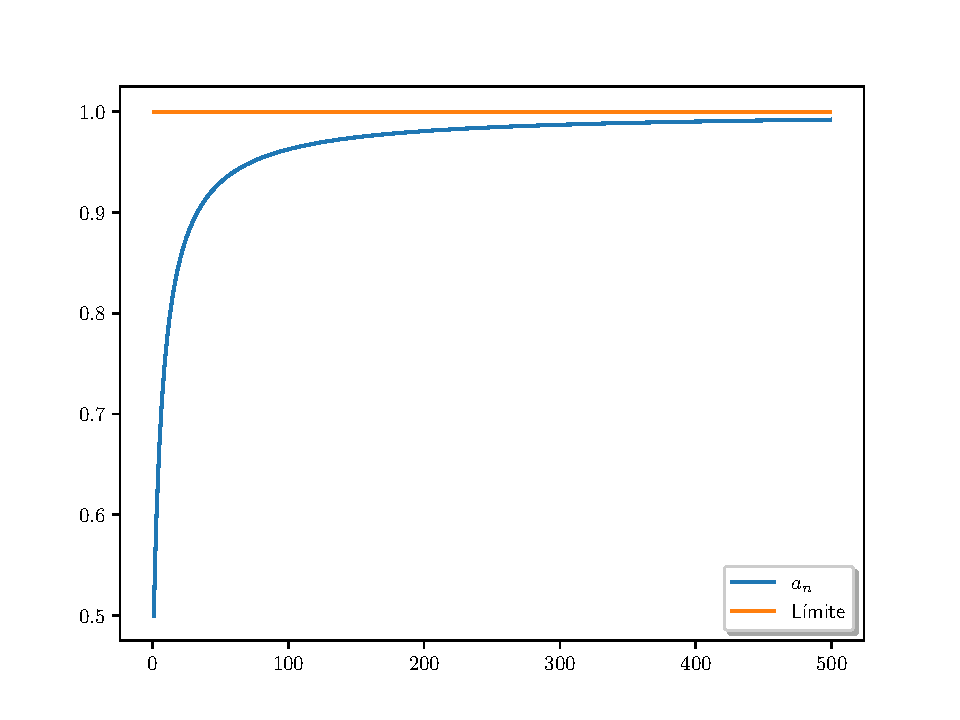
\includegraphics[width=7.5cm]{questions/p5}
        \end{figure}
    \end{minipage}
    \begin{minipage}{0.4\textwidth}
        \begin{listing}[H]
            \inputminted[
                fontsize=\scriptsize,
                breaklines,
            ]{python}{questions/p5.py}
        \end{listing}
    \end{minipage}
\end{frame}

\begin{frame}[fragile]
    \begin{solution}
        \begin{columns}
            \begin{column}{0.48\textwidth}
                \inputminted[fontsize=\tiny,firstline=3,lastline=6]{python}{questions/p5.py}

                \

                \inputminted[fontsize=\tiny,firstline=8,lastline=12]{python}{questions/p5.py}

            \end{column}
            \begin{column}{0.48\textwidth}
                \inputminted[fontsize=\tiny,firstline=14,lastline=18]{python}{questions/p5.py}
            \end{column}
        \end{columns}
    \end{solution}
\end{frame}

\begin{frame}
    \begin{solution}
        \begin{algorithm}[H]
            $A\leftarrow 1.0$\;
            $B\leftarrow 1.0$\;
            $p\leftarrow 0$\;
            \Mientras{\normalfont $\left(\left(A+1\right)-A\right)-1=0$}{
                $A\leftarrow 2\ast A$\;
                $p\leftarrow p+1$\;
                \Mientras{\normalfont $\left(\left(A+B\right)-A\right)-B\neq0$}{
                    $B\leftarrow B+1$\;
                }
            }
        \end{algorithm}
    \end{solution}
\end{frame}

\begin{frame}
    \begin{solution}
        Sea la longitud de palabra de $N=4$ bits, genere una tabla que muestre la representación decimal de los números $+7,+6,+5,+4,+3,+2,+1,+0,-0,-1,-2,-3,-4,-5,-6,-7$ y $-8$ en la representación de su signo-magnitud y complemento a dos.
        Es decir,

        \

        \begin{table}[ht!]
            \centering
            \begin{tabular}{|x{2.5cm}|x{2.5cm}|x{3.1cm}|}
                \hline
                Representación decimal & Representación signo-magnitud & Representación complemento a dos \\
                \hline$+7$             & $0111$                        & $0111$                           \\
                \hline
            \end{tabular}
        \end{table}
    \end{solution}
\end{frame}